\documentclass{beamer}
\label{key}\usetheme{Singapore}
\usepackage{dsfont}
\usepackage{multicol}
\usepackage{lmodern}
\usepackage{lipsum}
\usepackage{marvosym}
\usepackage{graphicx}
%\usepackage{ tipa }

\title{Nonlinear Observer for Tightly Coupled Integration of Pseudorange and Inertial Measurements}
\subtitle{Guide and Navigation Systems}
\author{P. Bramante, L. Bertoni, F. Di Luzio}
\institute{Universit\`a degli Studi di Pisa \\ Master's Degree in Robotics and Automation Engineering}
\date{\today}

\begin{document}
	
	\begin{frame}
	\titlepage
	\end{frame}	

    \AtBeginSection[]
	{
	
	\begin{frame}<beamer>
		\frametitle{Outline}
		\tableofcontents[currentsection]
	\end{frame}
}
%%%%%%%%%%%%%%%%%%%%%%%%%%%%%%%%%%%%%%%%%%%%%%%%%%%%%%%%%%%%%%%%%%%%%%%%%%%%%%%%%%%%%%%%%%%%%%%%%%%%%%%%%%%%%%%%%%%


\section{Introduction}
	\begin{frame}
		\frametitle{Introduction}
		This presentation shows the obtained results by the studying of the article written by Tor. A. Johansen and Thor I. Fossen.
		\vspace{0.5cm}
		
	\begin{figure}[H]
			\centering
			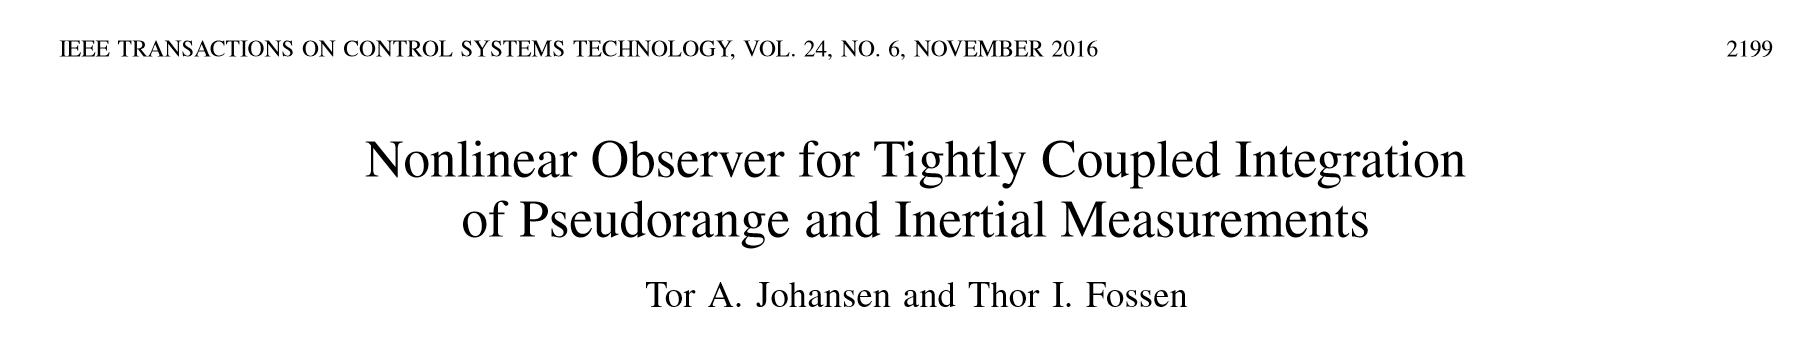
\includegraphics[scale=0.3]{title}
			%\caption{Block diagram of the closed-loop system for $\mu$ analysis and synthesis. \label{fig::title}}
		\end{figure}
	\end{frame}

	\begin{frame}
		\frametitle{Introduction}
	%	The work has been developed in Matlab and Simulink (v. R2016b).
	The goal of navigation system is to estimate the vehicle position within a certain area. The most common approach is to implement a inertial navigation system ($INS$), based on $IMU$ (Inertial Measurement Unit).\\
	\vspace{0.3cm}
	An $INS$ is a navigation system that calculates the position, the orientation and the velocity of a moving vehicle without the need for external references, by using a computer, motion sensors (accelerometers), rotation sensors (gyroscopes) and occasionally magnetic sensors (magnetometers).
	
	%Using an interconnection of a nonlinear attitude observer and a translational motion observer based on pseudorange and range-range measurements, a tightly coupled integrated aided inertial navigation system is designed!?!?!?\\
	
	%Due to the problem of measurements integration, this method is supported by other techniques. In this work, the inertial navigation system is aid by pseudorange measurements, obtained by transponders.
	%The article shows hot to build an inertial navigation  system  with the aid of pseudorange measurements, obtained by proper transponders.
	\end{frame}


	\begin{frame}
		\frametitle{Introduction}
		In order to estimate position, velocity and orientation, inertial sensors measurements have to been integrated.
		\[ p =  \int_0^t{(v+\beta) dt} = (\bar{v}+\beta) t \]
		\noindent
		Therefore sensor bias and noise effects diverge during time.\\
		To solve this problem, $INS$ is aid by other techniques, such as $GPS$, $range-range$ measurements, etc..
	\end{frame}

	\begin{frame}
		\frametitle{Introduction}
		Here the goal is to support $INS$ with $pseudorange$ measurements, obtained by transponders, and $nonlinear$ $observers$. 
		
		\begin{figure}[H]
			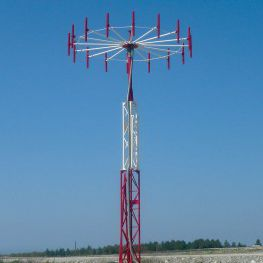
\includegraphics[scale=0.4]{transp}
		\end{figure}
	\end{frame}
	
	
	\begin{frame}
		\frametitle{Introduction}
    There are two main approaches to design nonlinear observer:
    
        \begin{itemize}
            
            \item $Loosely$ $Coupled$: range measurements are used to estimate position and velocity and given to the observer;
            \vspace{0.2cm}
            \item $Tightly$ $Coupled$: range measurements are directly used in a state observer together with inertial measurements.
        \end{itemize}
        \vspace{0.2cm}
        Here the second approach is applied.
    \end{frame}
	
	
	
	
%%%%%%%%%%%%%%%%%%%%%%%%%%%%%%%%%%%%%%%%%%%%%%%%%%%%%%%%%%%%%%%%%%%%%%%%%%%%%%%%%%%%%%%%%%%%%%%%%%%%%%%%%%%%%%%%%%%
\section{System Model}
    \subsection{Vehicle Kinematics}
	\begin{frame}
	\frametitle{Vehicle Kinematics}
	The vehicle kinematic model is given by
	
	\[ \dot{p^n} = v^n \]
	
	\[ \dot{v^n} = R^n_b f^b + g^n\]
	
	\[ \dot{R^n_b} = R^n_bS(\omega^b_{ib}) \]
	
	Where $p^n$, $v^n$, $f^n$ are position, velocity and proper acceleration in NED (North-East-Down), respectively, while the attitude is described by a rotation matrix $R^n_b$ that represents the rotation from \textit{body} to NED; $\omega^b_{ib}$ represents the rotation rate of body with respect to ECI (Earth-Centered-Inertial) and $g^n$ denotes the gravity vector. We also assume NED to be an inertial frame. 
	
	\end{frame}
 \subsection{Inertial Sensor Models}	
	\begin{frame}
	\frametitle{Inertial Sensor Models}
	The inertial sensor model is based on the strapdown assumption
	
	\[ f^b_{IMU} = f^b + \epsilon_f\]
	
	\[ \omega^b_{ib,IMU} = \omega^b_{ib} + b + \epsilon_\omega \]
	
	\[ \dot{b} = \epsilon_b \]
	
	\[ m^b_{mag} = m^b + \epsilon_m \]
	
	where $\epsilon_f$, $\epsilon_\omega$ and $\epsilon_m$ account for noise, and $b$ denotes the rate gyro bias that is driven by the noise $\epsilon_b$ and assumed to be bounded.  
	\\ All sensors are 3-D.
	\end{frame}

	\begin{frame}
	\frametitle{Pseudorange Measurement Model}
	The range is generally measured indirectly by some receiver that measures signal time of arrival, phase difference or other variables. The geometric range 
	
	\[ \rho_i = \|p^n - p^n_i\|_2 \]
	
	is a nonlinear function of the vehicle position $p^n$ and the $i$th transponder position $p^n_i$, given by their Euclidean distance.
	\end{frame}
\subsection{Pseudorange Measurement Model}
	\begin{frame}
		\frametitle{Pseudorange Measurement Model}
		The pseudorange measurement model is
		
		\[ y_i = \rho_i + \beta + \epsilon_{yi} \]
		
		where $\beta \in \mathds{R}$ is a bias parameter due to unknown clock synchronization errors or other unknown effects and $\epsilon_{yi}$ the noise.
		$i = 1,2,...,m$ where $m$ is the number of transponders.
	\end{frame}
	
	\begin{frame}
	\frametitle{Pseudorange Measurement Model}
	The nonlinear model can be approximated with a linear one by an algebraic transformation 
	
		\[ 2C_{\delta x}x = \delta + \varepsilon  \]
		
	where the matrix $C_{\delta x} \in \mathds{R}^{(m-1)\times4}$ is
	
	$$
	C_{\delta x} :=
	\begin{pmatrix}
	(p^n_m - p^n_1)^T & y_1 - y_m \\
	\vdots \\
	(p^n_m - p^n_{m-1})^T & y_{m-1} - y_m 
	\end{pmatrix} 
	$$
	
	$\varepsilon \in \mathds{R}^{m-1}$ the noise and $\delta \in \mathds{R}^{m-1}$ the vector of squared range measurements. \\ $x := (p^n_\Delta;\beta)$ where $p_\Delta^n = p^n - p^n_0$ ($p_0^n$ is a reference point in NED). 
	\end{frame}

	\begin{frame}
		\frametitle{Pseudorange Measurement Model}
		If $m \geqslant 5$ and if there is no measurement noise, the unique solution to
		\[ 2C_{\delta x} x = \delta + \epsilon \]
		is given by
		\[\hat{x} = \frac {C_{\delta x}^{+} \delta}{2}  \]
		where $\hat{x} := (\hat{p^n_\Delta};\hat{\beta})$ is an estimation of the vehicle position and of the clock bias.
\end{frame}
%%%%%%%%%%%%%%%%%%%%%%%%%%%%%%%%%%%%%%%%%%%%%%%%%%%%%%%%%%%%%%%%%%%%%%%%%%%%%%%%%%%%%%%%%%%%%%%%%%%%%%%%%%%%%%%%%%%
\section{Nonlinear Observers}
	\begin{frame}
	\frametitle{Nonlinear Observer}
	Two observer are designed: one for the attitude estimation and one for the translational motion estimation. 
		\begin{figure}[H]
		\centering
		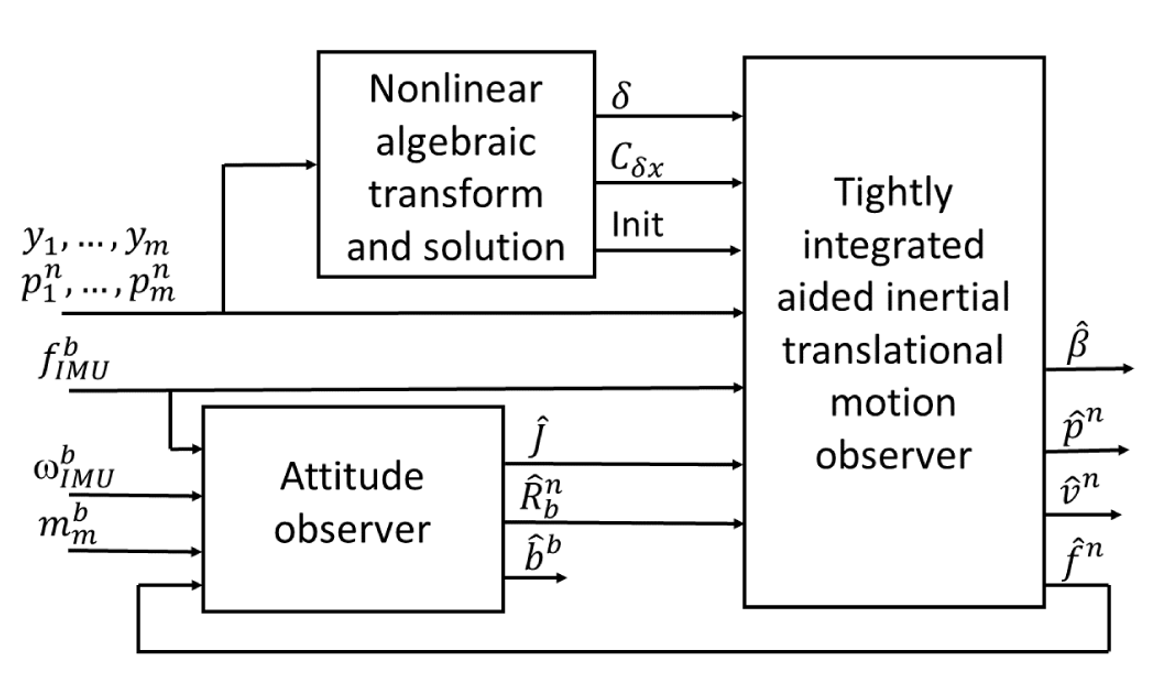
\includegraphics[scale=0.3]{observers}
	%	\caption{Overall block diagram for tightly integrated observer.}
	\end{figure}
	\end{frame}

	\begin{frame}
		\frametitle{Nonlinear Observer}
		The Attitude Observer ($AO$) should provide an estimation of the bias gyroscope, in order to \textit{clean} the angular velocity measurements, and of the rotation matrix from the body frame to the $NED$ frame.\\
		\vspace{0.3cm}
		The pseudorange model provides an initialisation of the translational motion observer ($TMO$) which should estimate position, velocity and acceleration of the vehicle and the clock bias of the transponders.
	\end{frame}
%%%%%%%%%%%%%%%%%%%%%%%%%%%%%%%%%%%%%%%%%%%%%%%%%%%%%%%%%
\subsection{Attitude Observer}

    \begin{frame}
        \frametitle{Attitude Observer}
    The $AO$ estimates the following variables    
        \[ \dot{\hat{R}}^n_b  =  \hat{R}^n_b S(\omega^b_{ib,IMU} - \hat{b}) + \sigma K_pJ(t, \hat{R}^n_b) \]      
        \[ \dot{\hat{b}} = Proj(-k_I vex(\mathds{P}_a (sat(\hat{R}^n_b)^T K_P J(t, \hat{R}^n_b))),M_{\hat{b}} )\]
        
        where $sat(\cdot)$ is an element-wise saturation, $vex(S(x)) = x$ and $k_I > 0$. $K_P > 0 \in \mathds{R}^{3\times 3}$ is a symmetric gain matrix, $\sigma \geq 1$.
       
        The second formula guarantees that the estimation of $b$ is bounded: 
        \[\|\hat{b} \|_2 \leqslant M_{\hat{b}} \]
        Every time $\hat{b}$ is available, this is subtracted to the gyroscope measurement.
        
    \end{frame}
    
%	\begin{frame}
%		\frametitle{Attitude Observer}
%		One of the variables to estimate is the gyroscope bias
		
%		\[ \dot{\hat{b}} = Proj(-k_I vex(\mathds{P}_a (sat(\hat{R}^n_b)^T K_P J(t, \hat{R}^n_b))),M_{\hat{b}} )\]
		
%		where $sat(\cdot)$ is an element-wise saturation, $vex(S(x)) = x$ and $k_I > 0$.\\
%		\vspace{0.3cm}
%		The formula guarantees that the estimation of is bounded: 
		
%		\[\|\hat{b} \|_2 \leqslant M_{\hat{b}} \]	
%	\end{frame}



%	\begin{frame}
%		\frametitle{Attitude Observer}
%		The second variable to estimate is the rotation matrix $R^n_b$.
		
%		\[ \dot{\hat{R}}^n_b  =  \hat{R}^n_b S(\omega^b_{ib,IMU} - \hat{b}) + \sigma K_pJ(t, \hat{R}^n_b)       \]
		
%		\vspace{0.3cm}
%		where $K_P > 0 \in \mathds{R}^{3\times 3}$ is a symmetric gain matrix, $\sigma \geq 1$.\\ 
%		\vspace{0.3cm}
%		Every time $\hat{b}$ is available, this is subtracted to the gyroscope measurement.\\
%	\end{frame}


	\begin{frame}
 		\frametitle{Attitude Observer}
 		The function $J(\cdot) \in  \mathds{R}^{3\times 3}$ is a stabilizing injection term that acts as an angular velocity when the discrepancy between measured vectors in body frame, here specific force and magnetic field from the accelerometer and the magnetometer, with the corresponding one in $NED$ frame.
 		
 		\[ J(t, \hat{R}^n_b)  = (E^n - \hat{R}^n_b E^b)(E^b)^T   \]

 		

	\end{frame}

	\begin{frame}
		\frametitle{Attitude Observer}
		%$E^n$,$E^b \in \mathds{R}^{3\times 3}$
		
		\[ E^b = (q_1^b, S(q^b_1)q_2^b, S^2(q_1^b)q_2^b)    \]
		
		\[ E^n = (q_1^n, S(q^n_1)q_2^n, S^2(q_1^n)q_2^n)    \]
		
		
		\[ q_1^b = m^b_{mag}/\|m^b_{mag}\|_2 \qquad q_2^b = f^b_{IMU}/\|g^n\|_2    \]
		
		\[ q_1^n = m^n/\|m^n\|_2 \qquad q_2^n = \hat{f}^n/\|g^n\|_2    \]
		
	\end{frame}
%%%%%%%%%%%%%%%%%%%%%%%%%%%%%%%%%%%%%%%%%%%%%%%%%%%%%%%%%%%%
\subsection{Translational Motion Observer}

	\begin{frame}
		\frametitle{Translational Motion Observer}
		The $TMO$ estimates $p^n$, $v^n$, $f^n$, $\beta$.
		
		\[ \dot{\hat{p}}^n_\Delta = \hat{v}^n + K_{pp}(\delta - \hat{\delta})  \]
		
		\[ \dot{\hat{\beta}} = K_{\beta p} (\delta - \hat{\delta}) \]
		
		\[ \dot{\hat{v}}^n = \hat{f}^n + g^n + K_{vp}(\delta - \hat{\delta})\]
		
		\[ \dot{\xi} = - \sigma K_P J(t, \hat{R}^n_b)f^b_{IMU} + K_{\xi p}(\delta - \hat{\delta}) \]
		
		\[ \hat{f}^n = \hat{R}^n_b f^b_{IMU} + \xi  \]
		
		where $\hat{\delta} = 2C_{\delta x}\hat{x}$ and the gain matrix $K \in \mathds{R}^{10\times(m-1)}$ is made of the matrices $K_*$ and is in general time varying.
	\end{frame}

	\begin{frame}
		\frametitle{Translational Motion Observer}
		The injection term is provided by
		
		\[  \delta - \hat{\delta} \]
		where
		\begin{itemize}
			\item $\delta$ is computed by the pseudorange model;
			\item $\hat{\delta}$ by the TMO.
		\end{itemize}
	
	For each variable to estimate, the injection term is weighted by a gain $K_{ij}$.		
	\end{frame}

	\begin{frame}
		\frametitle{Translational Motion Observer}
		The gain matrix $K$ is time varying and calculated as
		
		\[ K := PC^TR^{-1} \]
		
		where $P$ is solution of the $Riccati$ equation
		
		\[ \dot{P} = PA + A^TP - PC^TR^{-1}CP + Q\]
	\end{frame}

%	\begin{frame}
	%	\frametitle{Translational Motion Observer}
	%	The $TMO$ equations can be written in matrix form,
	%	Then it is possible to build the \textit{estimated state} vector $\dot{\tilde{\chi}} = (\tilde{p}^n_\Delta;\tilde{\beta}; \tilde{\hat{v}}^n; \tilde{\hat{f}}^n) \in \mathds{R}^{10}$ and the relative LTV error system
		
	%	\[ \dot{\tilde{\chi}} = (A - KC)\tilde{\chi} + Bu + B\epsilon_u + K\varepsilon\]
		
	%	\[ u = \tilde{R}^n_b \dot{f}^b + \tilde{R}^n_b S(\omega^b_{ib})f^b - \hat{R}^n_b S(\tilde{b})f^b\]
%	\end{frame}

	\begin{frame}
		\frametitle{Translational Motion Observer}
		The matrices $A \in \mathbb{R}^{10\times 10}$,$B \in \mathbb{R}^{10\times 3}$,$C \in \mathds{R}^{(m-1) \times 10} $ and $K \in \mathds{R}^{10 \times (m-1)}$ are described as follows
		$$
		A :=
		\begin{pmatrix}
		0 & 0 & I_3 & 0 \\ 
		0 & 0 & 0 & 0 \\
		0 & 0 & 0 & I_3 \\
		0 & 0 & 0 & 0
		\end{pmatrix}
		\qquad
		B := 
		\begin{pmatrix}
		0 \\ 0 \\ 0 \\ I_3
		\end{pmatrix}
		$$
		
		$$
		K := 
		\begin{pmatrix}
		K_{pp} \\ K_{\beta p} \\ K_{vp} \\ K_{\xi p}
		\end{pmatrix}
		\qquad
		C :=
		\begin{pmatrix}
		2C_{\delta x} & 0 & 0
		\end{pmatrix}
		$$
	\end{frame}

%%%%%%%%%%%%%%%%%%%%%%%%%%%%%%%%%%%%%%%%%%%%%%%%%%%%%%%%%%%%%%%%%%%%%%%%%%%%%%%%%%%%%%%%%%%%%%%%%%%%%%%%%%%%%%%%%%%	
\section{Implementation}	
	\begin{frame}
		\frametitle{Implementation}
		The whole model has been implemented with MATLAB/Simulink (R2016b).
		\\
		\vspace{0.5cm}
		In the following each observer is presented in terms of structure and results, i.e. the difference between the true value of the vehicle position and of the bias parameter and their estimation.
	\end{frame}
	
	\begin{frame}
		\frametitle{Implementation}
		Data used by the authors are \\
		\begin{itemize}
			\item pseudorange measurements obtained by radio beacons;
			\item accelerations and angular velocities by IMU. 
		\end{itemize}
		\vspace{0.5cm}
		The inertial sensor model is based on the strapdown assumption, i.e. the inertial measurement unit is fixed to the body frame.
	\end{frame}
	
	\begin{frame}
		\frametitle{Data Generation}
		In order to generate data the $6DOF$ Simulink block has been used
		\begin{figure}[H]
			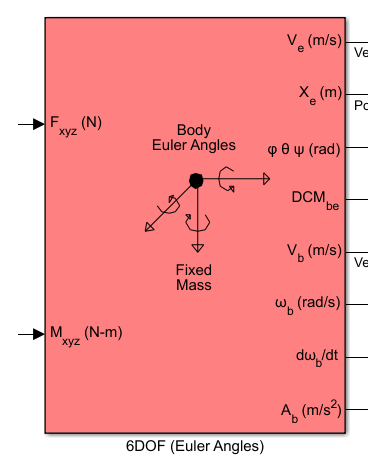
\includegraphics[scale=0.4]{6DOF}
		\end{figure}
	\end{frame}
	
	\begin{frame}
		\frametitle{Data Generation}
		\begin{itemize}
			\item The real position of the vehicle is given from $X_e(m)$;
			\item The range measurements always by $X_e(m)$ but corrupted by noise;
			\item Specific forces from $A_b(m/s^2)$;
			\item Angular velocities from $\omega_b(rad/s)$.
		\end{itemize}
	\end{frame}

	\begin{frame}
		\frametitle{Simulink Model}
	
		\begin{figure}[H]
			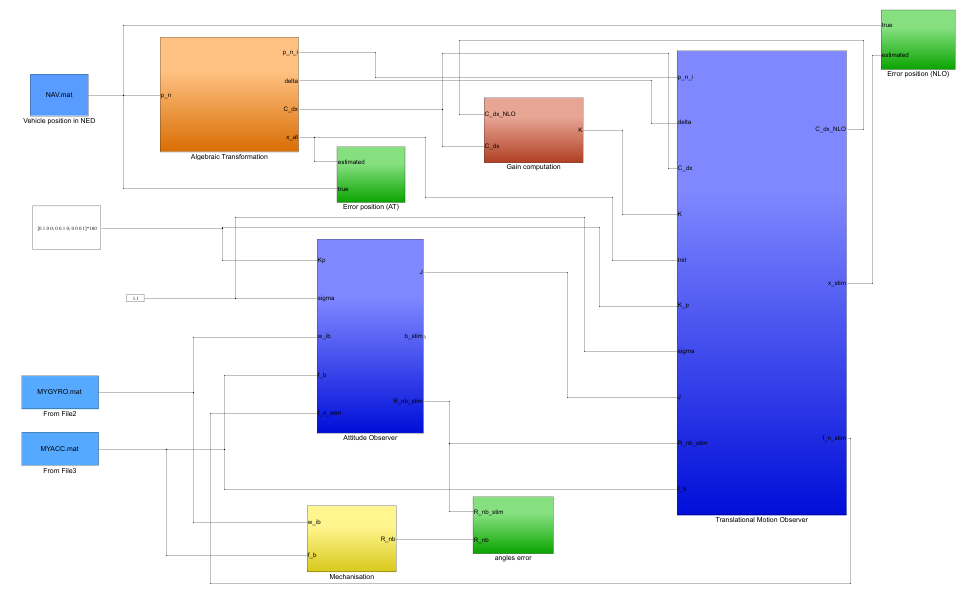
\includegraphics[scale=0.3]{continuous_mod.png}
		\end{figure}
	\end{frame}





\section{Results}
    \begin{frame}
        \frametitle{Results}
        In this section, the results of the Nonlinear Observer
        are presented in terms of committed error between the
        true and estimated state.
        %our experiments/simulations we assume
        The transponder positions and the observer
        tuning have been decided by
        a \textit{trial and error} approach.
    \end{frame}

 \begin{frame}
        \frametitle{Results}
        The following picture shows the transponder positions
        and the real trajectory to be estimated.
        
        \begin{columns}
            \column{.4\textwidth}
        Transponder positions $p_i^n$, $i=1,2,.. 6$
        \begin{matrix}
            p_1^n& =& [100;0;0.1] \\
            p_2^n& =& [0;100;10] \\
            p_3^n &=& [100;100;20] \\
            p_4^n &=& [300;150;50] \\
            p_5^n &=& [500;660;60] \\
            p_6^n &=& [400;800;100]
        \end{matrix}
			\column{.6\textwidth}
			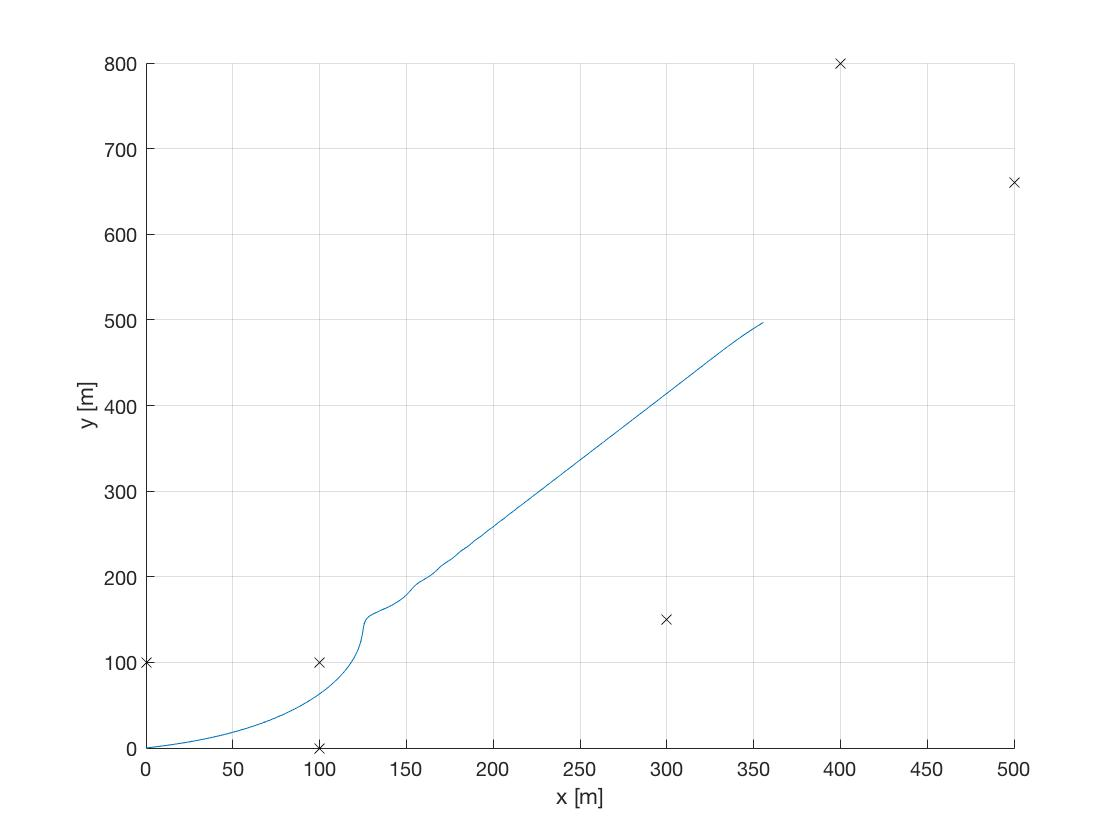
\includegraphics[scale=0.15]{true_traj.jpg}
		\end{columns}
        
    \end{frame}


    
    \begin{frame}
        \frametitle{Pseudorange Model Design}
        The Pseudorange Model has been implemented 
        with positions obtained directly from the 
        previously described equations,
        without modelling the receiver on the vehicle that
        receives signals from transponders
    \end{frame}





	\begin{frame}
		\frametitle{Pseudorange Model Results}
		\begin{itemize}
		       \item Position and bias errors
		\end{itemize}
		\begin{columns}
			\column{.3\textwidth}
			%\begin{figure}
			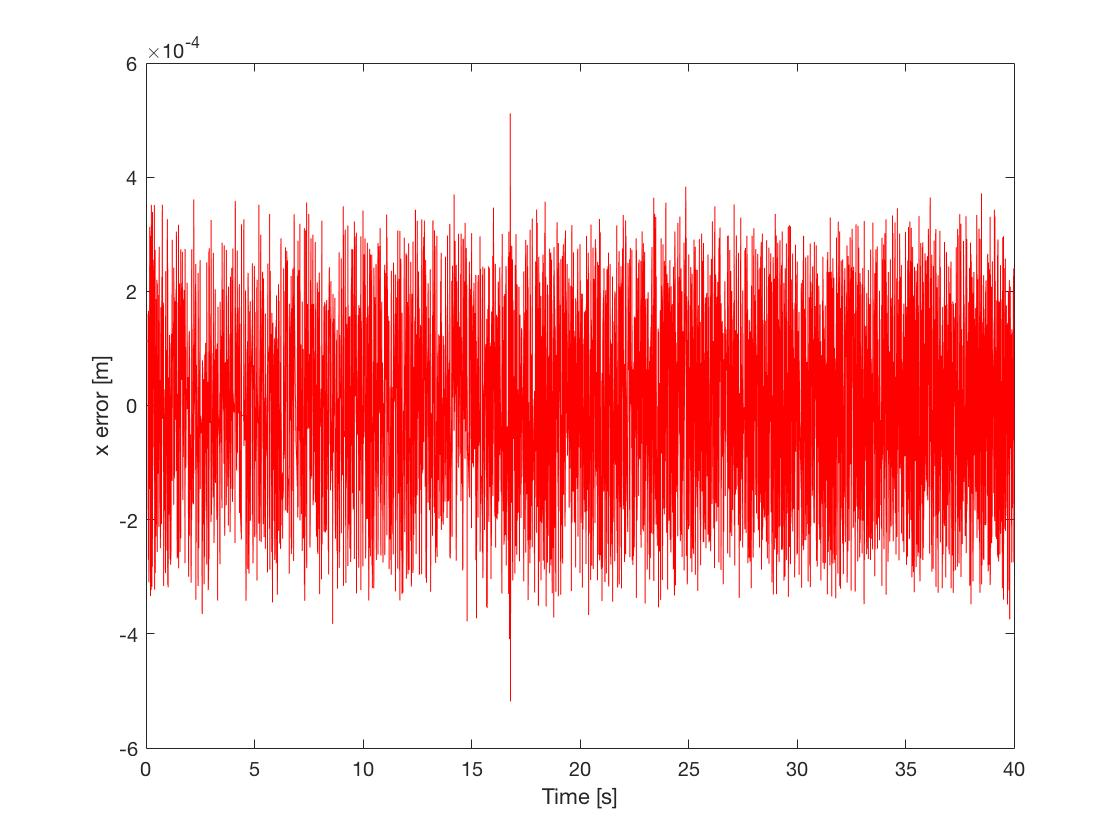
\includegraphics[scale= 0.1]{x_error.jpg}\\
			%\caption{\small{X error.}}
			%\end{figure}
			%\begin{figure}
			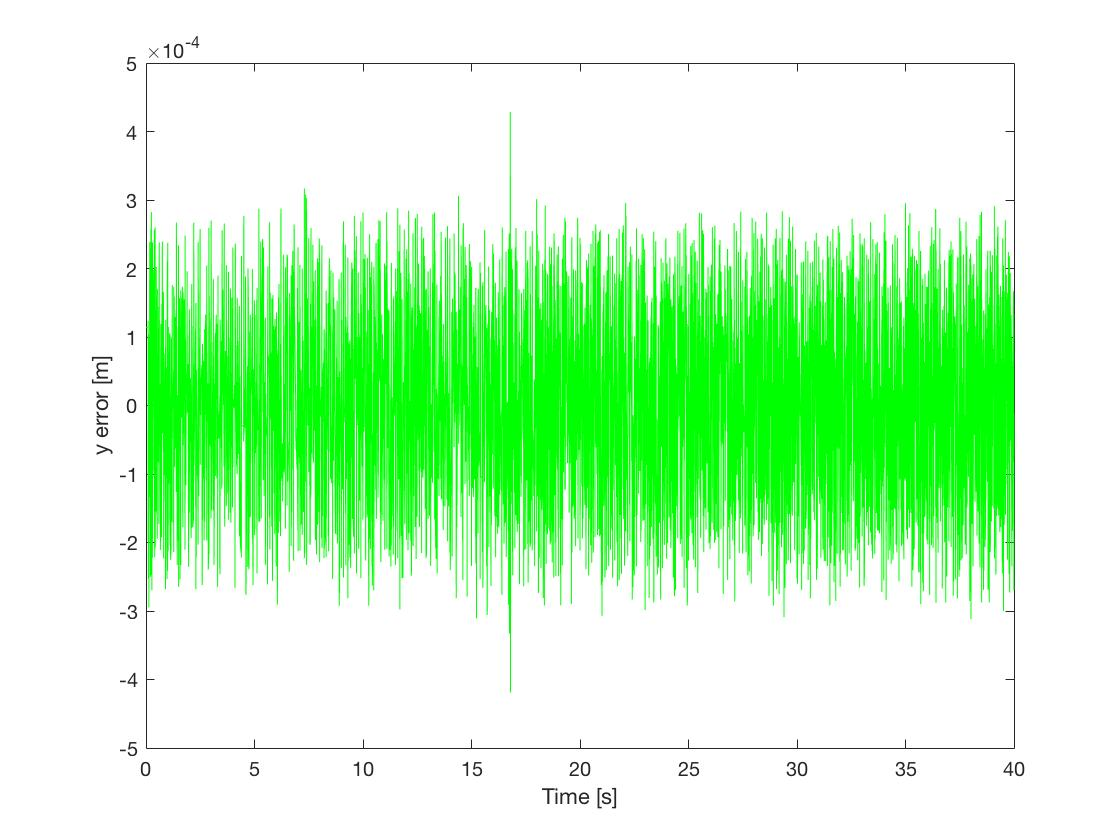
\includegraphics[scale=0.1]{y_error.jpg}
			%\caption{\small{Y error.}}
			%\end{figure}
			\column{.3\textwidth}
			\centering
			%\begin{figure}
			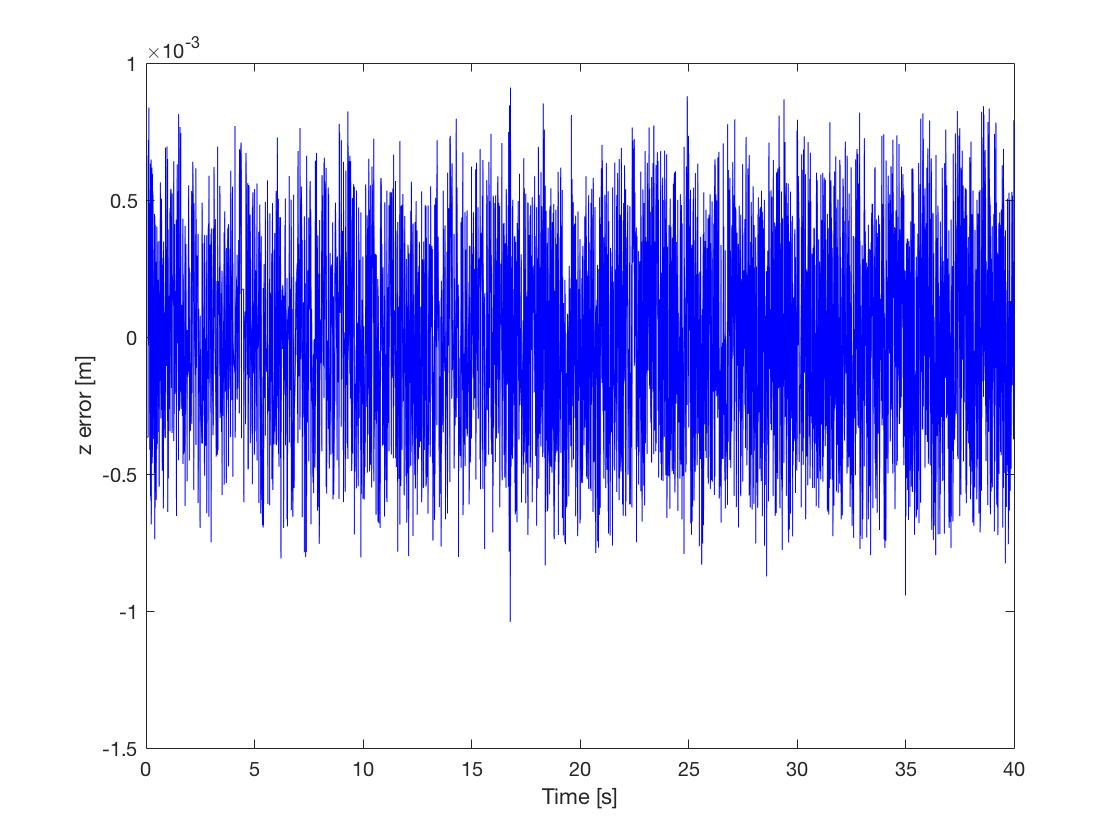
\includegraphics[scale= 0.1]{z_error.jpg}\\
			%\caption{\small{Z error.}}
			%\end{figure}
			%\begin{figure}
			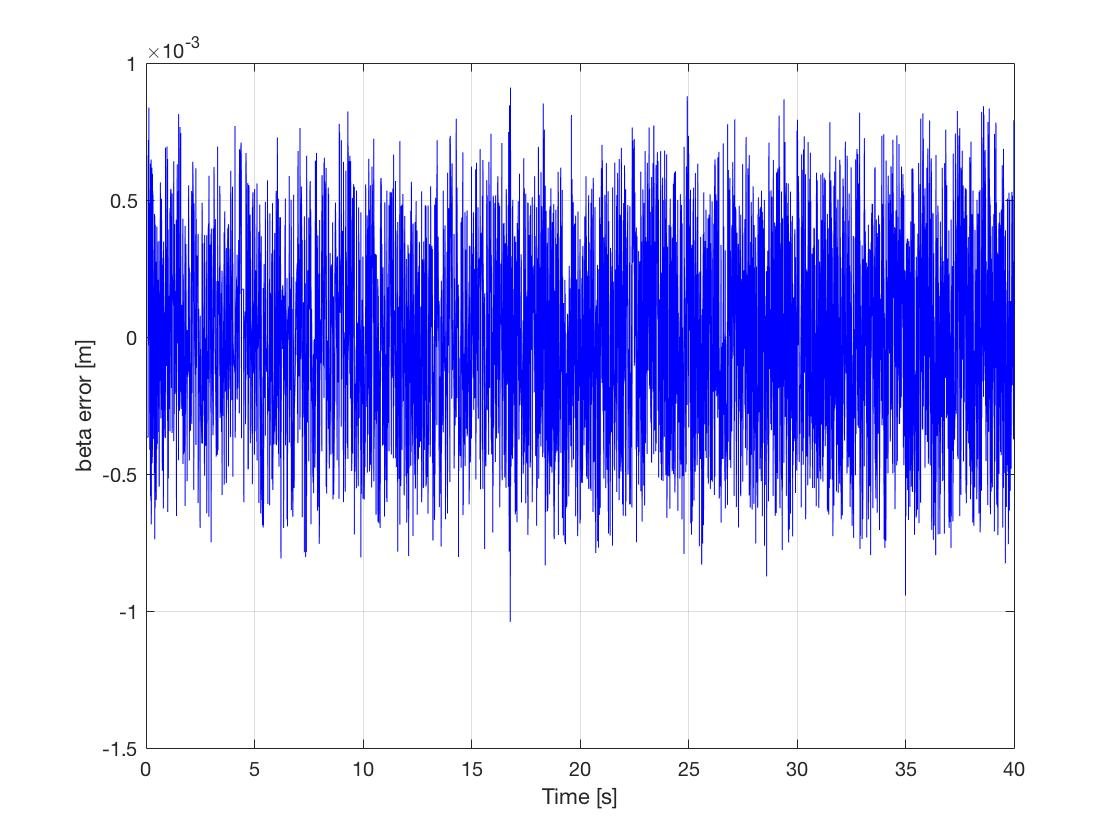
\includegraphics[scale= 0.1]{beta_error.jpg}
			%\caption{\small{$\beta$ error.}}
			%\end{figure}
		\end{columns}
	\end{frame}

		
		
	%\begin{frame}
	%	\frametitle{Implementation Design}
	%	The $AO$ is made of three main function blocks:\\
	%	\begin{itemize}
	%		\item $J\_computation$ computes the stabilizing injection term;
			
	%		\item $b\_computation$ computes the estimation of the gyroscope bias;
			
	%		\item $Rot\_func$ computes an estimation of the rotation matrix $R_b^n$.
	%	\end{itemize}
%	\end{frame}

	\begin{frame}
		\frametitle{$AO$ Results}
		\begin{itemize}
		       \item Angles errors
		\end{itemize}
		% angles error and norm of Rnb
		\begin{columns}[t]
			\column{.5\textwidth}
			\centering
			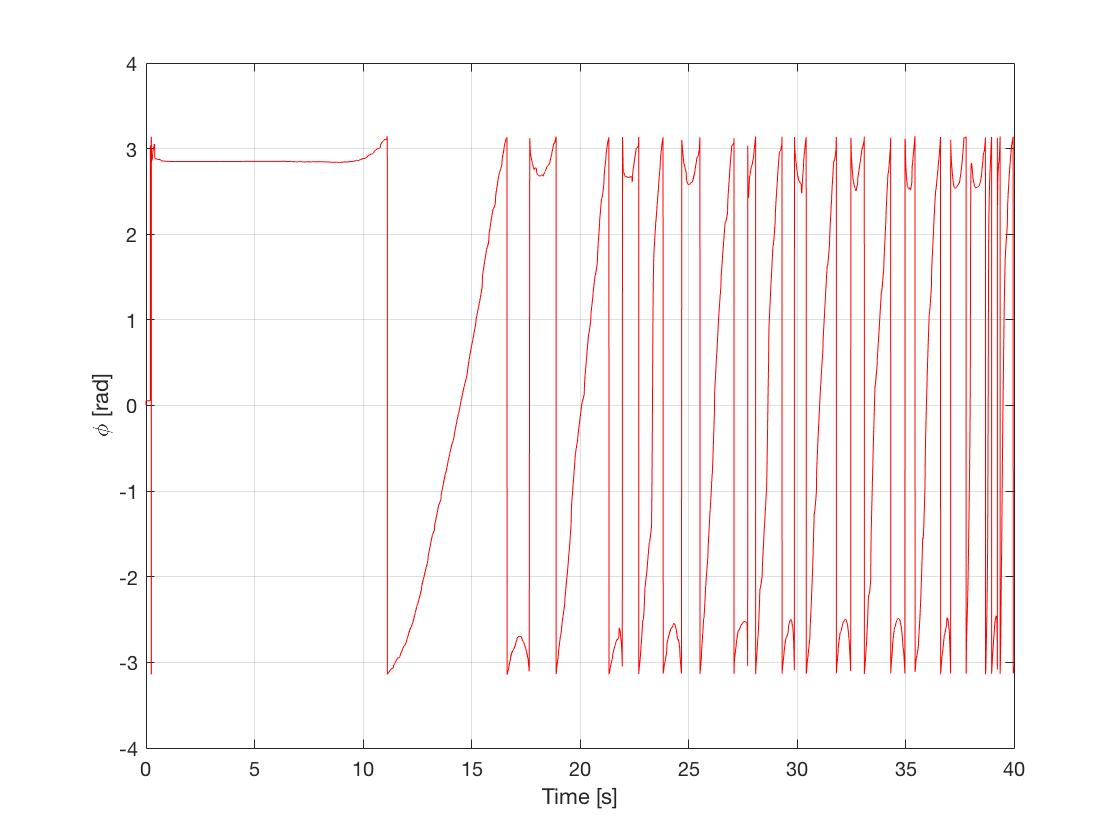
\includegraphics[scale= 0.12]{phi_angle.jpg}\\
			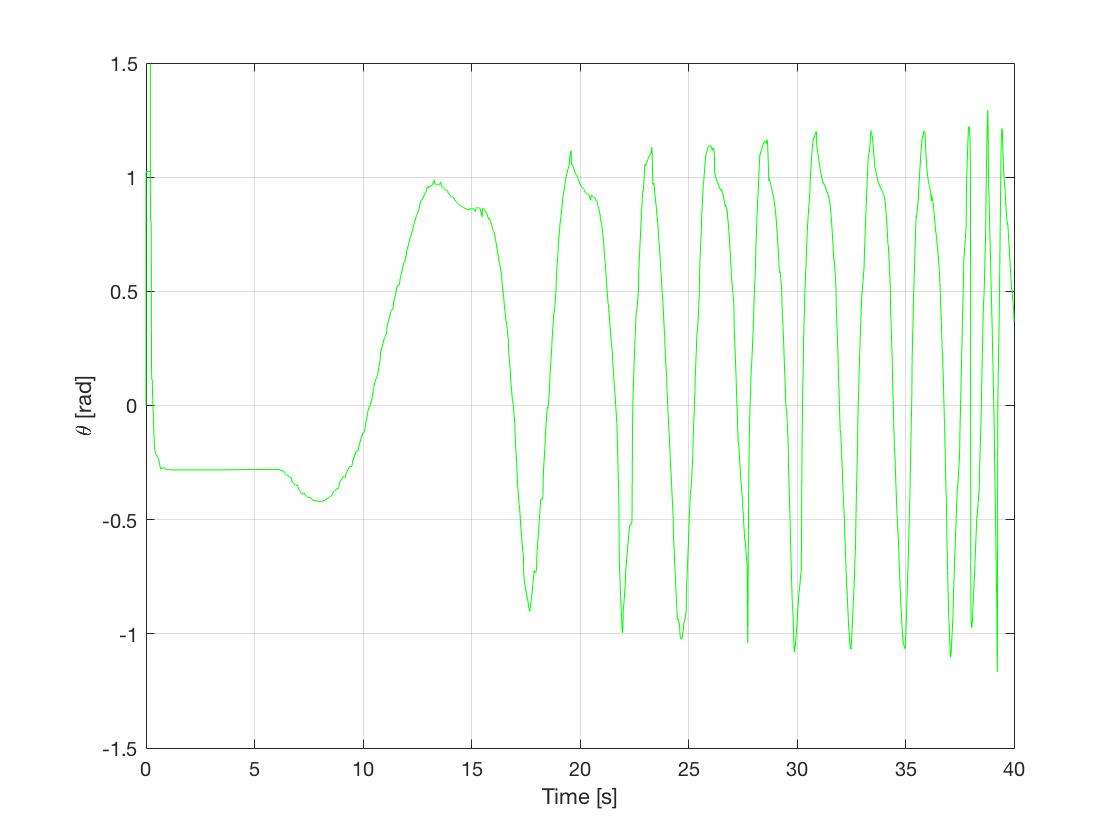
\includegraphics[scale= 0.12]{theta_angle.jpg}
			\column{.5\textwidth}
			\centering
			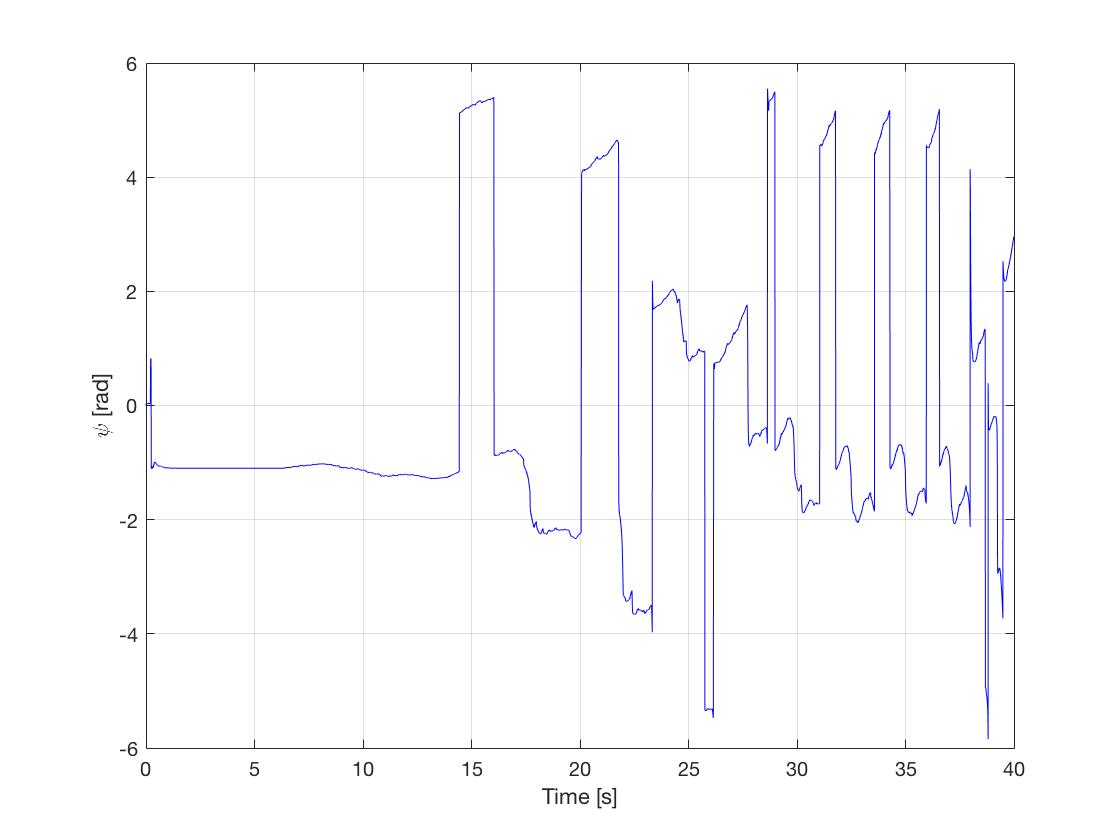
\includegraphics[scale= 0.12]{psi_angle.jpg}\\
			\vspace{0.4cm}
			Whatever tuning does not allow to have a good estimation of the angles, in terms of error respect to the true ones.
		\end{columns}
	\end{frame}
	

	\begin{frame}
		\frametitle{$AO$ Results}
		
		\begin{figure}[H]
			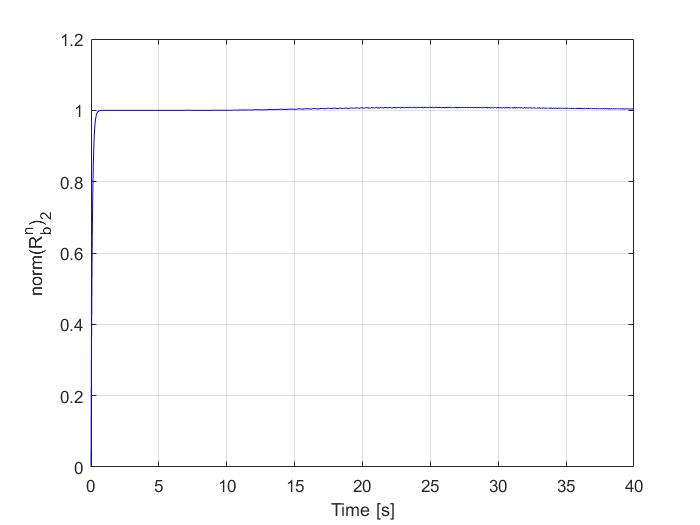
\includegraphics[scale=0.4]{norm_rot}
		\end{figure}
		
	\end{frame}


    \begin{frame}
		\frametitle{$TMO$ Results}
		Despite of the non-estimation of $AO$,
		the $TMO$ provides a good position estimation
		only for a
		simulation time of about 50s.
		
		\[ \dot{\hat{p}}^n_\Delta = \hat{v}^n + K_{pp}(\delta - \hat{\delta})  \]
		
		
		At the beginning, the weighted injection term 
		$K_{pp}(\delta - \hat{\delta})$ prevails on 
		$\hat{v}^n$. Then $\hat{v}^n$ prevails and brings
		a bad estimation due to the fact that depends on
		$AO$.
		
	\end{frame}


   \begin{frame}
		\frametitle{$TMO$ Results}
		\begin{itemize}
		    \item This situation is shown in the following figures.
	    \end{itemize}
		\begin{columns}[t]
			\column{.5\textwidth}
			\centering
			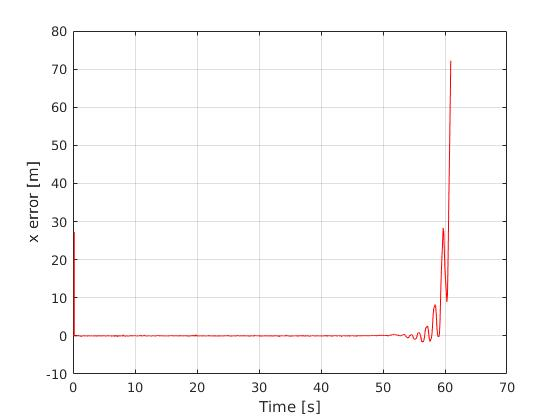
\includegraphics[scale=0.2]{x_div}\\
			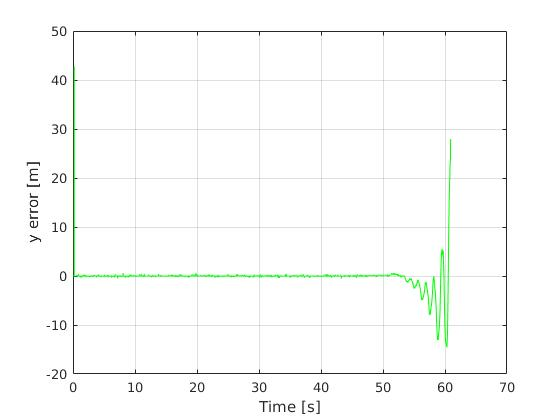
\includegraphics[scale=0.2]{y_div}
			\column{.5\textwidth}
			\centering
			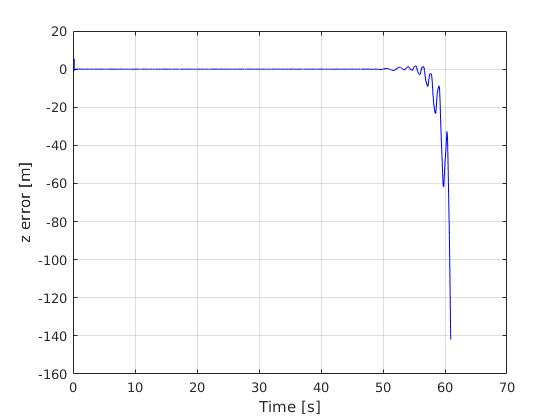
\includegraphics[scale=0.2]{z_div.jpg}\\
			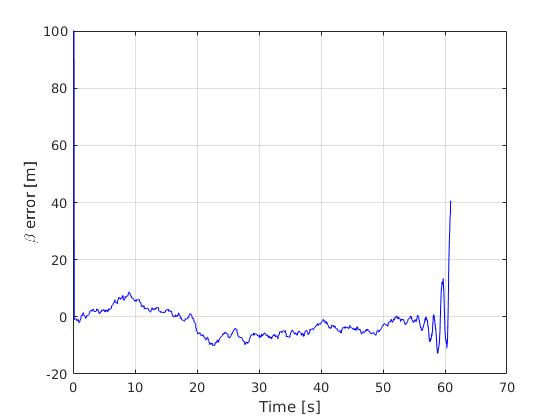
\includegraphics[scale=0.2]{beta_div.jpg}
		\end{columns}
		
	\end{frame}



	
	\begin{frame}
	\frametitle{$TMO$ Results}
	% position and beta error
	% no initial error
	\begin{itemize}
		\item No initial error.
	\end{itemize}
		\begin{columns}[t]
			\column{.5\textwidth}
			\centering
			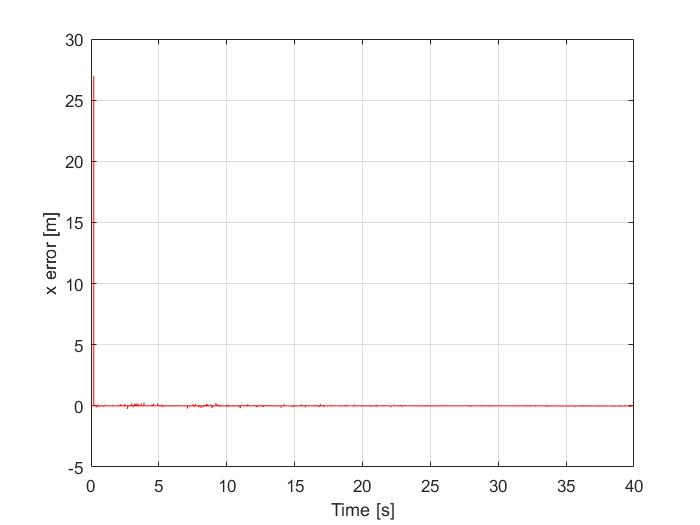
\includegraphics[scale=0.18]{nlo_x_0}\\
			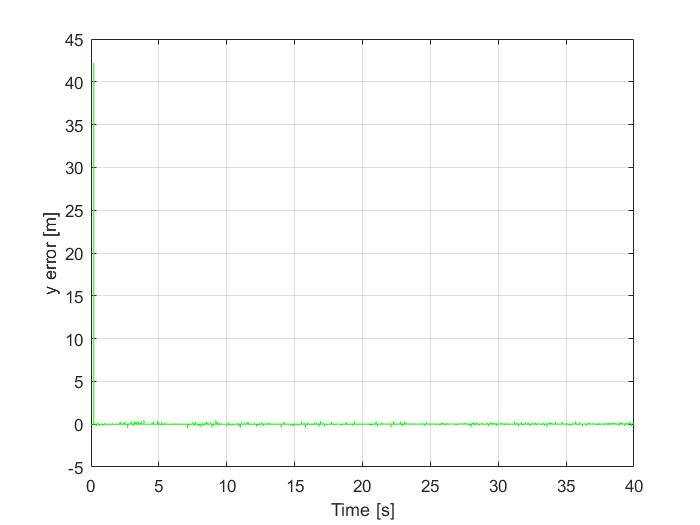
\includegraphics[scale=0.18]{nlo_y_0}
			\column{.5\textwidth}
			\centering
			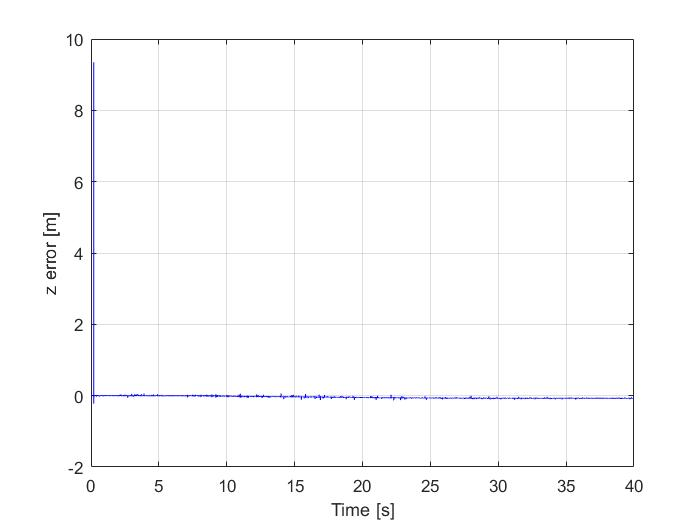
\includegraphics[scale=0.18]{nlo_z_0}\\
			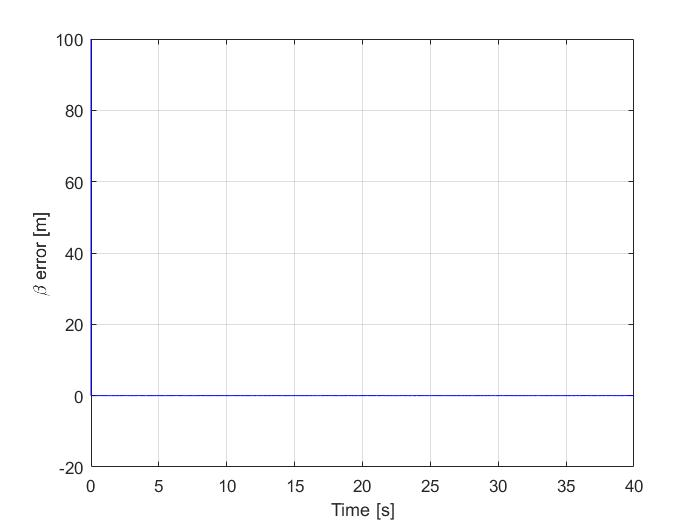
\includegraphics[scale=0.18]{nlo_beta_0}
		\end{columns}
	\end{frame}


	\begin{frame}
		\frametitle{$TMO$ Results}
			% position and beta error
			% no initial error
			\begin{itemize}
				\item Initial error [40;30;0;100].
			\end{itemize}
			\begin{columns}[t]
				\column{.5\textwidth}
				\centering
				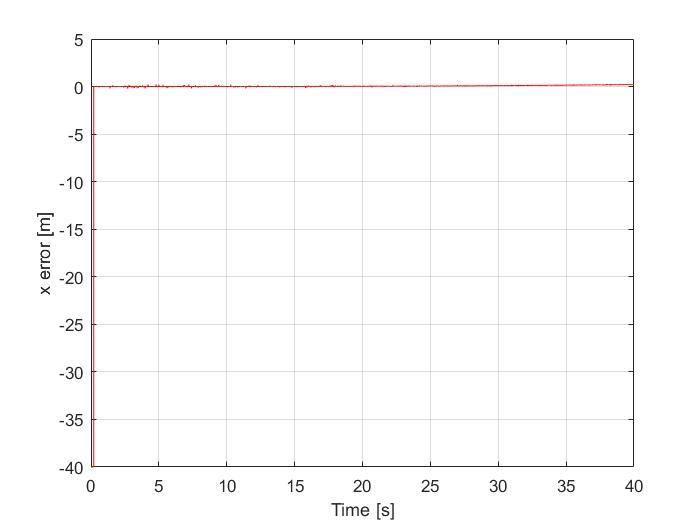
\includegraphics[scale=0.18]{nlo_x_1}\\
				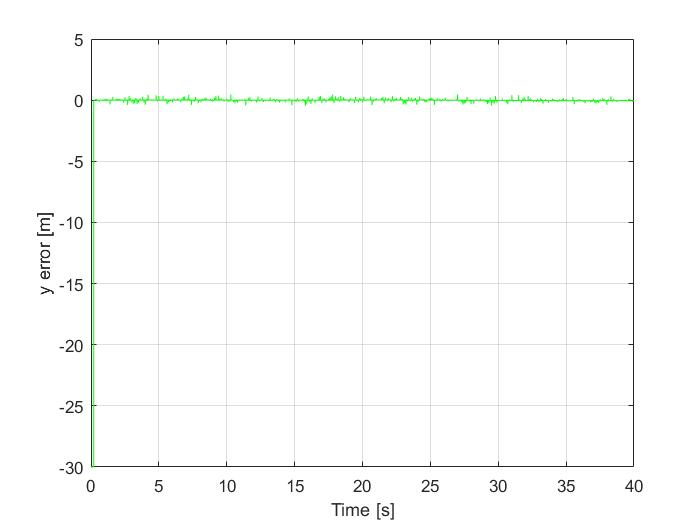
\includegraphics[scale=0.18]{nlo_y_1}
				\column{.5\textwidth}
				\centering
				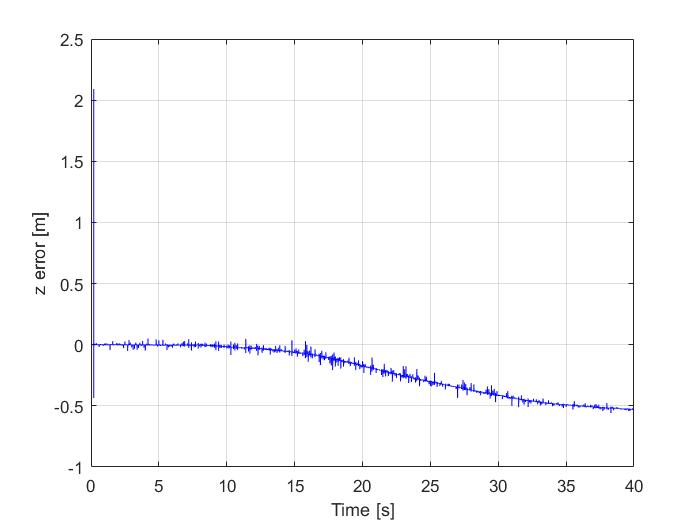
\includegraphics[scale=0.18]{nlo_z_1}\\
				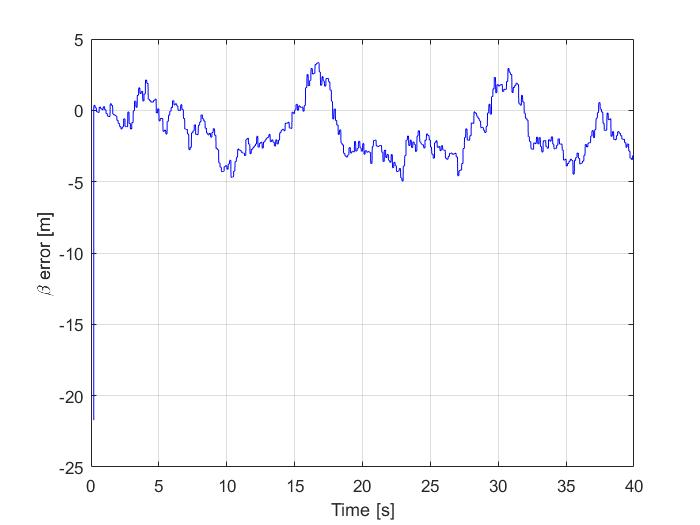
\includegraphics[scale=0.18]{nlo_beta_1}
			\end{columns}
	\end{frame}



	\begin{frame}
		\frametitle{$TMO$ Results}
		% position and beta error
		\begin{itemize}
			\item Initial error [250;0;0;0].
		\end{itemize}
		\begin{columns}[t]
			\column{.5\textwidth}
			\centering
			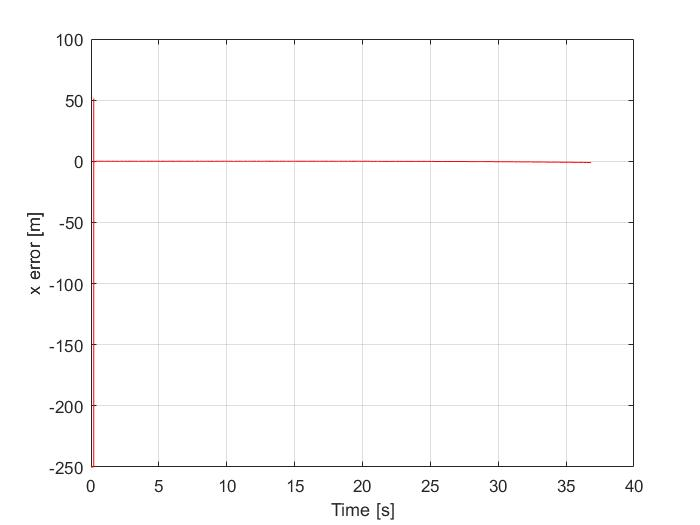
\includegraphics[scale=0.18]{nlo_x_2}\\
			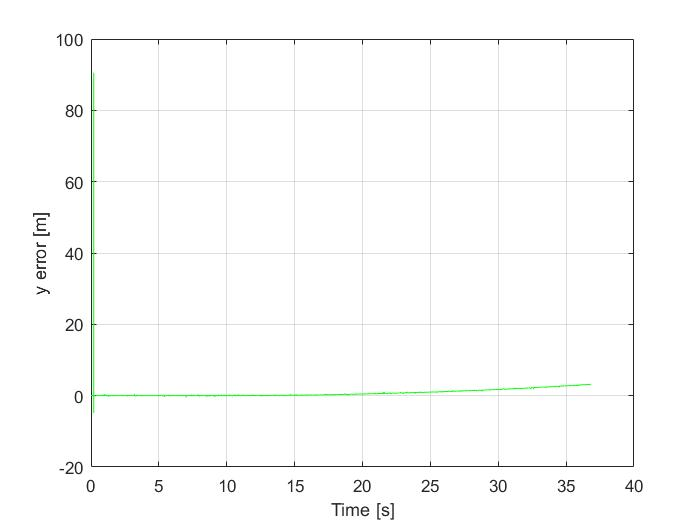
\includegraphics[scale=0.18]{nlo_y_2}
			\column{.5\textwidth}
			\centering
			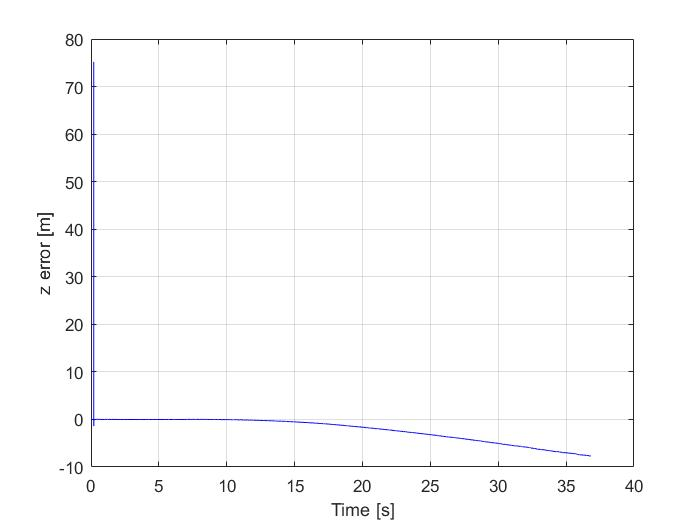
\includegraphics[scale=0.18]{nlo_z_2}\\
			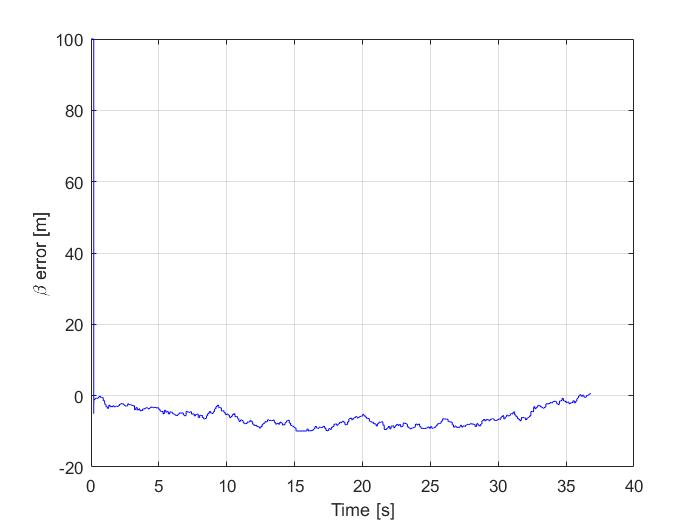
\includegraphics[scale=0.18]{nlo_beta_2}
		\end{columns}
	\end{frame}


	\begin{frame}
		\frametitle{$TMO$ Results}
		% position and beta error
		\begin{itemize}
			\item Initial error [100;50;0;100].
		\end{itemize}
		\begin{columns}[t]
			\column{.5\textwidth}
			\centering
			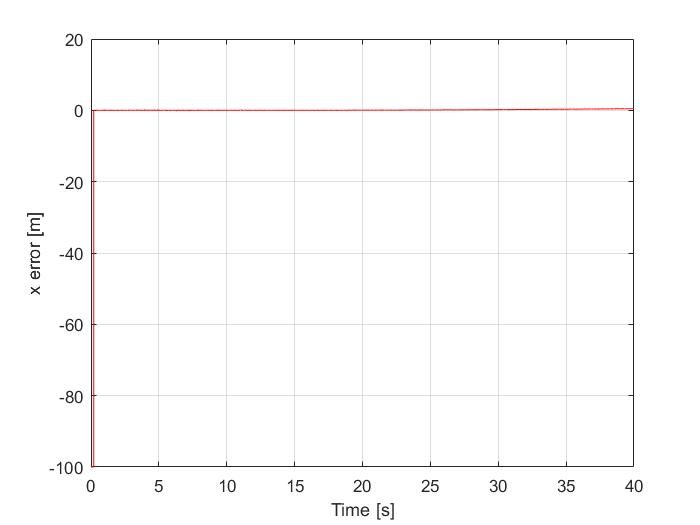
\includegraphics[scale=0.18]{nlo_x_3}\\
			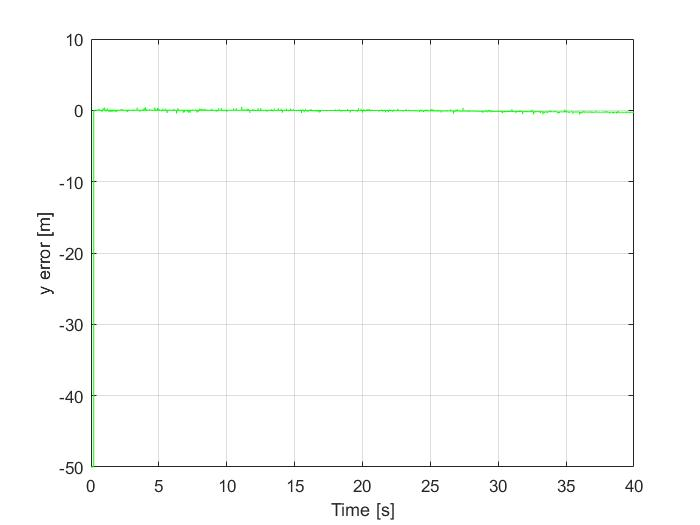
\includegraphics[scale=0.18]{nlo_y_3}
			\column{.5\textwidth}
			\centering
			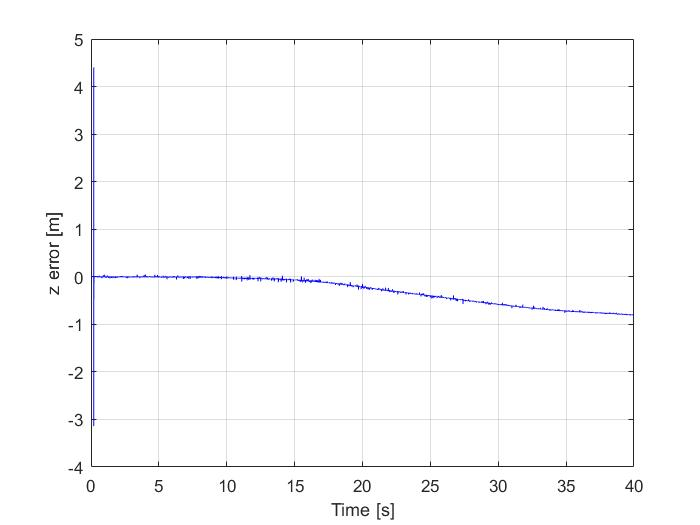
\includegraphics[scale=0.18]{nlo_z_3}\\
			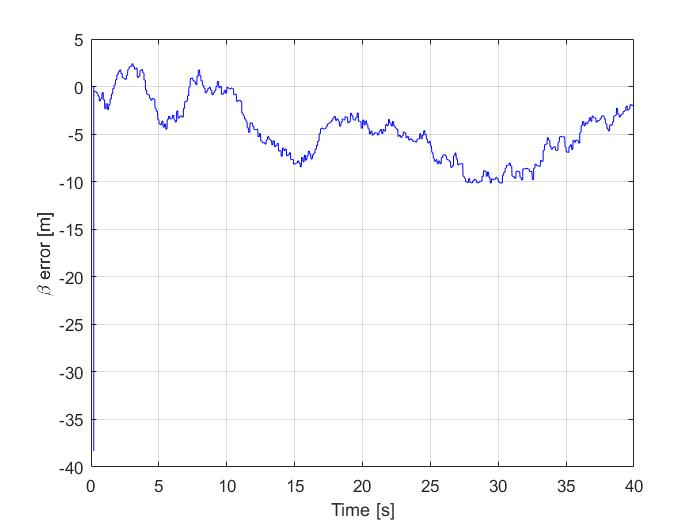
\includegraphics[scale=0.18]{nlo_beta_3}
		\end{columns}
	\end{frame}

	\begin{frame}
		\frametitle{$TMO$ Results}
		Comparison between real and estimated trajectory.
		\\
		\begin{columns}
			\column{.5\textwidth}
			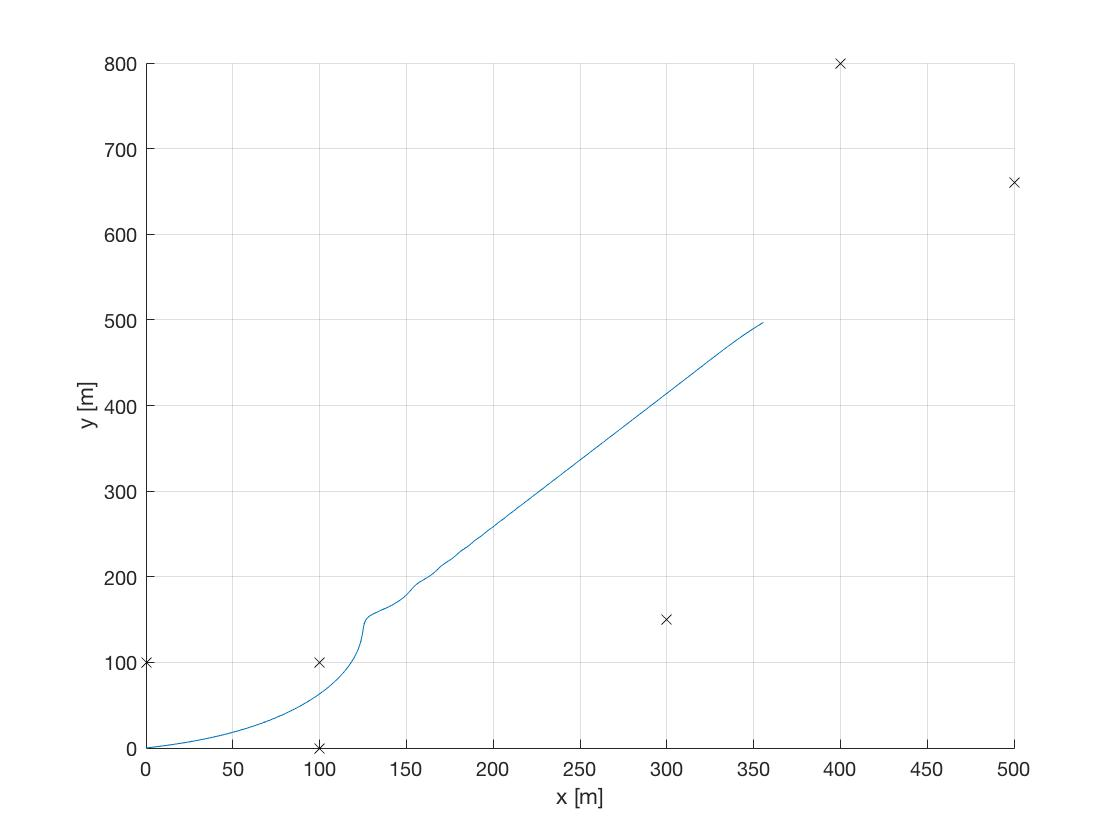
\includegraphics[scale=0.15]{true_traj.jpg}
			\column{.5\textwidth}
			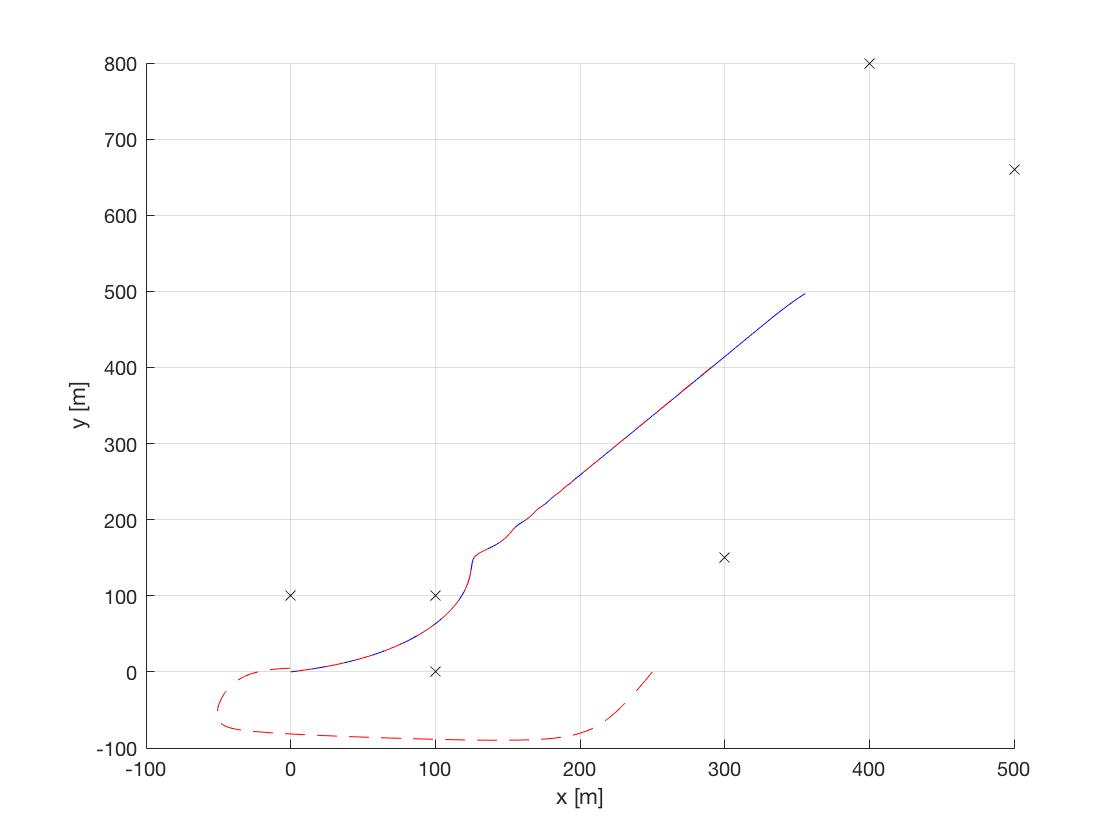
\includegraphics[scale=0.15]{comp_traj.jpg}
		\end{columns}
	\end{frame}
	
%	\begin{frame}
	%	\frametitle{Implementation Design}
	%	The estimates obtained by the Translational Motion Observer are then sent to a block that implements the Kalman-Bucy Filter in order to make a better estimation
		
	%	\begin{figure}[H]
	%		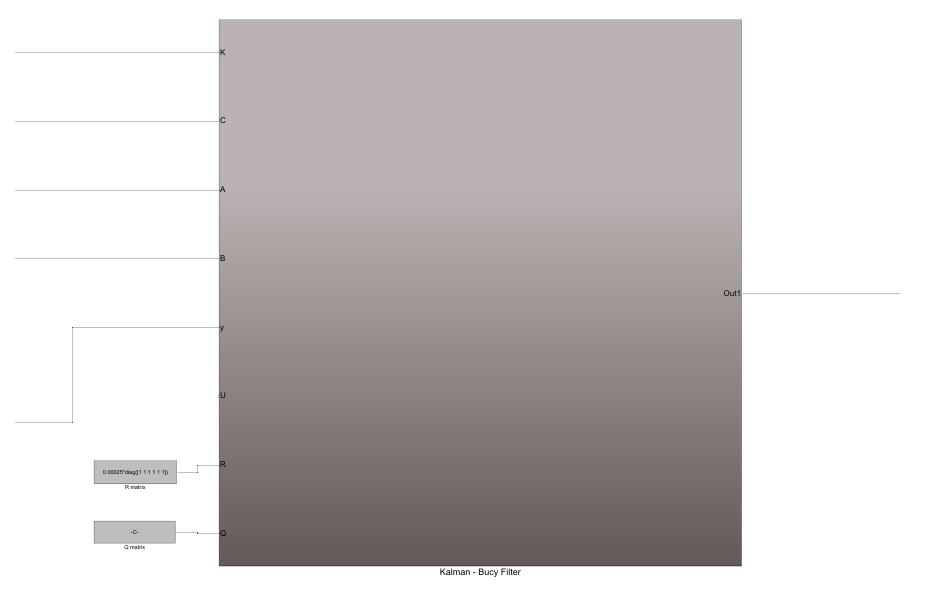
\includegraphics[scale=0.3]{KBF}
	%	\end{figure}	
%	\end{frame}
	
	%\begin{frame}
	%	Kalman Equations
	%\end{frame}
	
%	\begin{frame}
	%		figures
%	\end{frame}
	
	%\begin{frame}
	%		Confronto tra gli osservatori
	%\end{frame}
	
\section{Problems}
\subsection{Unbounded Covariance matrix $P$}
	\begin{frame}
		\frametitle{Unbounded $P$}
		Due to the time varying system and/or to the non-well-posedness, the covariance matrix $P$ is unbounded.
		\begin{figure}[H]
			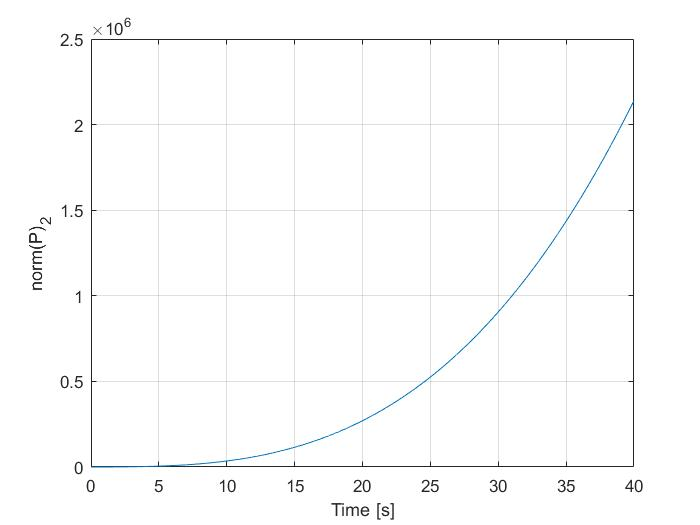
\includegraphics[scale=0.3]{pric}
		\end{figure} 
	\end{frame}

	\begin{frame}
		\frametitle{Bounded $K$}
		Despite that, the gain matrix $K$ results bounded.
		\begin{columns}[t]
			\column{.5\textwidth}
			\centering
			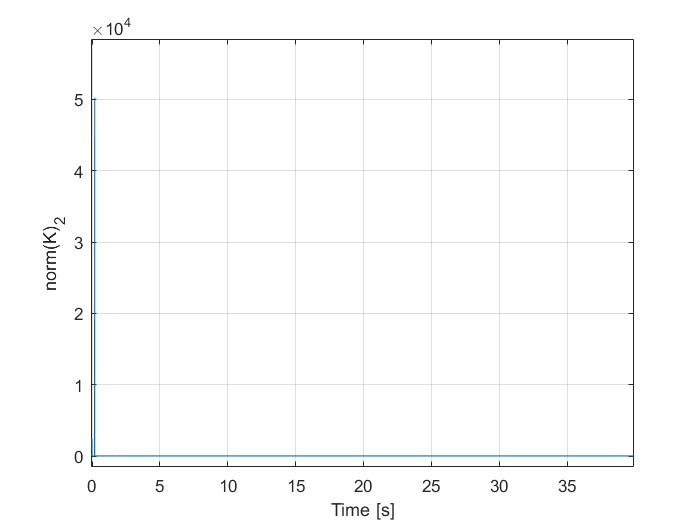
\includegraphics[scale=0.25]{kric}\\
			\column{.5\textwidth}
			\centering
			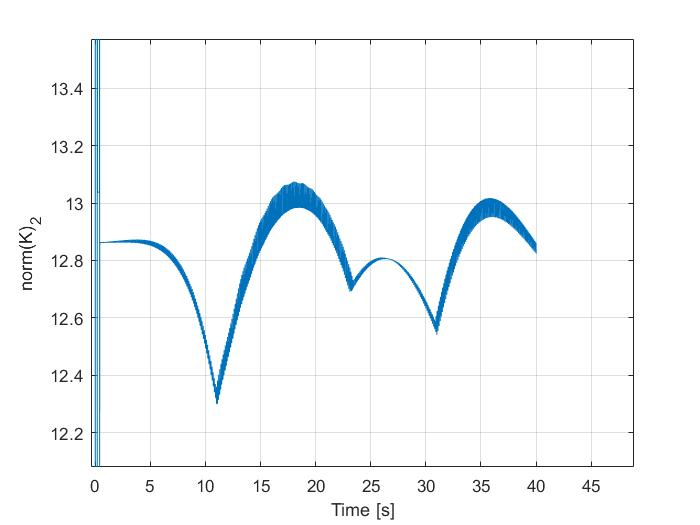
\includegraphics[scale=0.25]{kric2}\\
		\end{columns}
	\end{frame}
	
	\section{Conclusions}
		\begin{frame}
		\frametitle{Conclusions}
		This presentation has shown the results
		obtained by studying and implementation
		of a Nonlinear Observer for Tightly Coupled Integration
		of Pseudorange and Inertial Measurements
		designed by T.A. Johansen and T.I. Fossen.
		%The results show that the estimation error converges 
		%for a simulation time of about 50s.
		%After that the
		
		\end{frame}

\end{document}